\providecommand{\main}{./report}
\documentclass[../main.tex]{subfiles}
\begin{document}


\section{Experiment line-up}\label{section:appendix-experiment-lineup}

\renewcommand\theadalign{bl}
\begin{table}[ht]
    \centering
    \begin{tabular}{| l | l | l | l | l | l | l |}
    \hline
    \thead{Name method} & \thead{Classif-\\ication} & \thead{Regr-\\ ession} & \thead{Multi-\\output} & \thead{Feature \\ importance} & \thead{Feature\\support} & \thead{Feature\\ranking} \\
    \hline
    ANOVA F-value (\href{https://scikit-learn.org/stable/modules/generated/sklearn.feature_selection.f_classif.html}{sklearn}) & \checkmark & \checkmark &  & \checkmark &  &  \\ 
    \hline
    Boruta \citep{kursa_feature_2010} & \checkmark &  &  &  & \checkmark & \checkmark \\ 
    \hline
    Chi-Squared (\href{https://scikit-learn.org/stable/modules/generated/sklearn.feature_selection.chi2.html}{sklearn}) & \checkmark &  &  & \checkmark &  &  \\ 
    \hline
    Decision Tree (\href{https://scikit-learn.org/stable/modules/generated/sklearn.tree.DecisionTreeClassifier.html}{sklearn}) & \checkmark & \checkmark & \checkmark & \checkmark &  &  \\ 
    \hline
    FeatBoost (\href{https://github.com/amjams/FeatBoost}{github}) & \checkmark &  &  & \checkmark & \checkmark &  \\ 
    \hline
    Infinite Selection \citep{roffo_infinite_2015} & \checkmark &  &  & \checkmark &  & \checkmark \\ 
    \hline
    MultiSURF \citep{urbanowicz_benchmarking_2018} & \checkmark & \checkmark &  & \checkmark &  &  \\ 
    \hline
    Mutual Info \citep{zaffalon_robust_2014} & \checkmark & \checkmark &  & \checkmark &  &  \\ 
    \hline
    ReliefF \citep{urbanowicz_benchmarking_2018} & \checkmark & \checkmark &  & \checkmark &  &  \\ 
    \hline
    Stability Selection \citep{meinshausen_stability_2009} & \checkmark &  &  & \checkmark & \checkmark &  \\ 
    \hline
    TabNet \citep{arik_tabnet_2020} & \checkmark & \checkmark & \checkmark & \checkmark &  &  \\ 
    \hline
    XGBoost \citep{chen_xgboost_2016} & \checkmark & \checkmark &  & \checkmark &  &  \\ 
    \hline     
    \end{tabular}
    \caption{Feature Ranker line-up. Both classifiers and regressors are considered, as well as multioutput estimators.}
    \label{table:experiments-ranker-specification}
\end{table}



\renewcommand\theadalign{bl}
\begin{table}[ht]
    \centering
    \begin{tabular}{| l | l | l | l | l | l | l |}
    \hline
    \thead{Name dataset} & \thead{$n$} & \thead{$p$} & \thead{Task} & \thead{Multi-\\output} & \thead{Domain} & \thead{Group} \\
    \hline
    \makecell[tl]{Boston house \\prices} & 506 & 11 & Regression & No & Finance & - \\ 
    \hline
    Additive & 10000 & 10 & Regression & Yes & Synthetic & Chen et al. \citep{chen_learning_2018} \\ 
    \hline
    Orange & 10000 & 10 & Regression & Yes & Synthetic & Chen et al. \citep{chen_learning_2018} \\ 
    \hline
    XOR & 10000 & 10 & Regression & Yes & Synthetic & Chen et al. \citep{chen_learning_2018} \\ 
    \hline
    \makecell[tl]{Climate Model \\Simulation} & 540 & 18 & Classification & No & Nature & OpenML-CC18 \citep{bischl_openml_2019} \\ 
    \hline
    Cylinder bands & 5456 & 24 & Classification & No & Mechanics & OpenML-CC18 \citep{bischl_openml_2019} \\ 
    \hline
    Iris Flowers & 150 & 4 & Classification & No & Nature & - \\ 
    \hline
    Madelon & 2600 & 500 & Classification & No & Synthetic & Guyon \citep{guyon_design_2003} \\ 
    \hline
    Multifeat Pixel & 2000 & 240 & Classification & No & OCR & OpenML-CC18 \citep{bischl_openml_2019} \\ 
    \hline
    Nomao & 34465 & 89 & Classification & No & Geodata & OpenML-CC18 \citep{bischl_openml_2019}\\ 
    \hline
    Ozone Levels & 2534 & 72 & Classification & No & Nature & OpenML-CC18 \citep{bischl_openml_2019} \\ 
    \hline
    Phoneme & 5404 & 5 & Classification & No & Biomedical & OpenML-CC18 \citep{bischl_openml_2019} \\ 
    \hline
    Synclf easy & 10000 & 20 & Classification & No & Synthetic & Synclf \\ 
    \hline
    Synclf hard & 10000 & 50 & Classification & No & Synthetic & Synclf \\ 
    \hline
    Synclf medium & 10000 & 30 & Classification & No & Synthetic & Synclf \\ 
    \hline
    Synclf very hard & 10000 & 50 & Classification & No & Synthetic & Synclf \\ 
    \hline
    Synreg easy & 10000 & 10 & Regression & No & Synthetic & Synreg \\ 
    \hline
    Synreg hard & 10000 & 20 & Regression & No & Synthetic & Synreg \\ 
    \hline
    Synreg medium & 10000 & 10 & Regression & No & Synthetic & Synreg \\ 
    \hline
    Synreg hard & 10000 & 20 & Regression & No & Synthetic & Synreg \\ 
    \hline
    Texture & 5500 & 40 & Classification & No & \makecell[tl]{Pattern \\Recognition} & OpenML-CC18 \citep{bischl_openml_2019} \\ 
    \hline
    \makecell[tl]{Wall Robot \\Navigation} & 5456 & 24 & Classification & No & Mechanics & OpenML-CC18 \citep{bischl_openml_2019} \\ 
    \hline
    \end{tabular}
    \caption{All datasets considered in the experiment. Both real-world and synthetic datasets are considered. Whereas synthetic datasets are generated in the pipeline itself, real-world datasets are fetched from OpenML.}
    \label{table:experiments-dataset-specification}
\end{table}



\begin{figure}[ht]
    % https://colab.research.google.com/drive/1l4a_IOkiYfFDd5Q5bvAtMvBLRZ2iQEwP
    \centering
    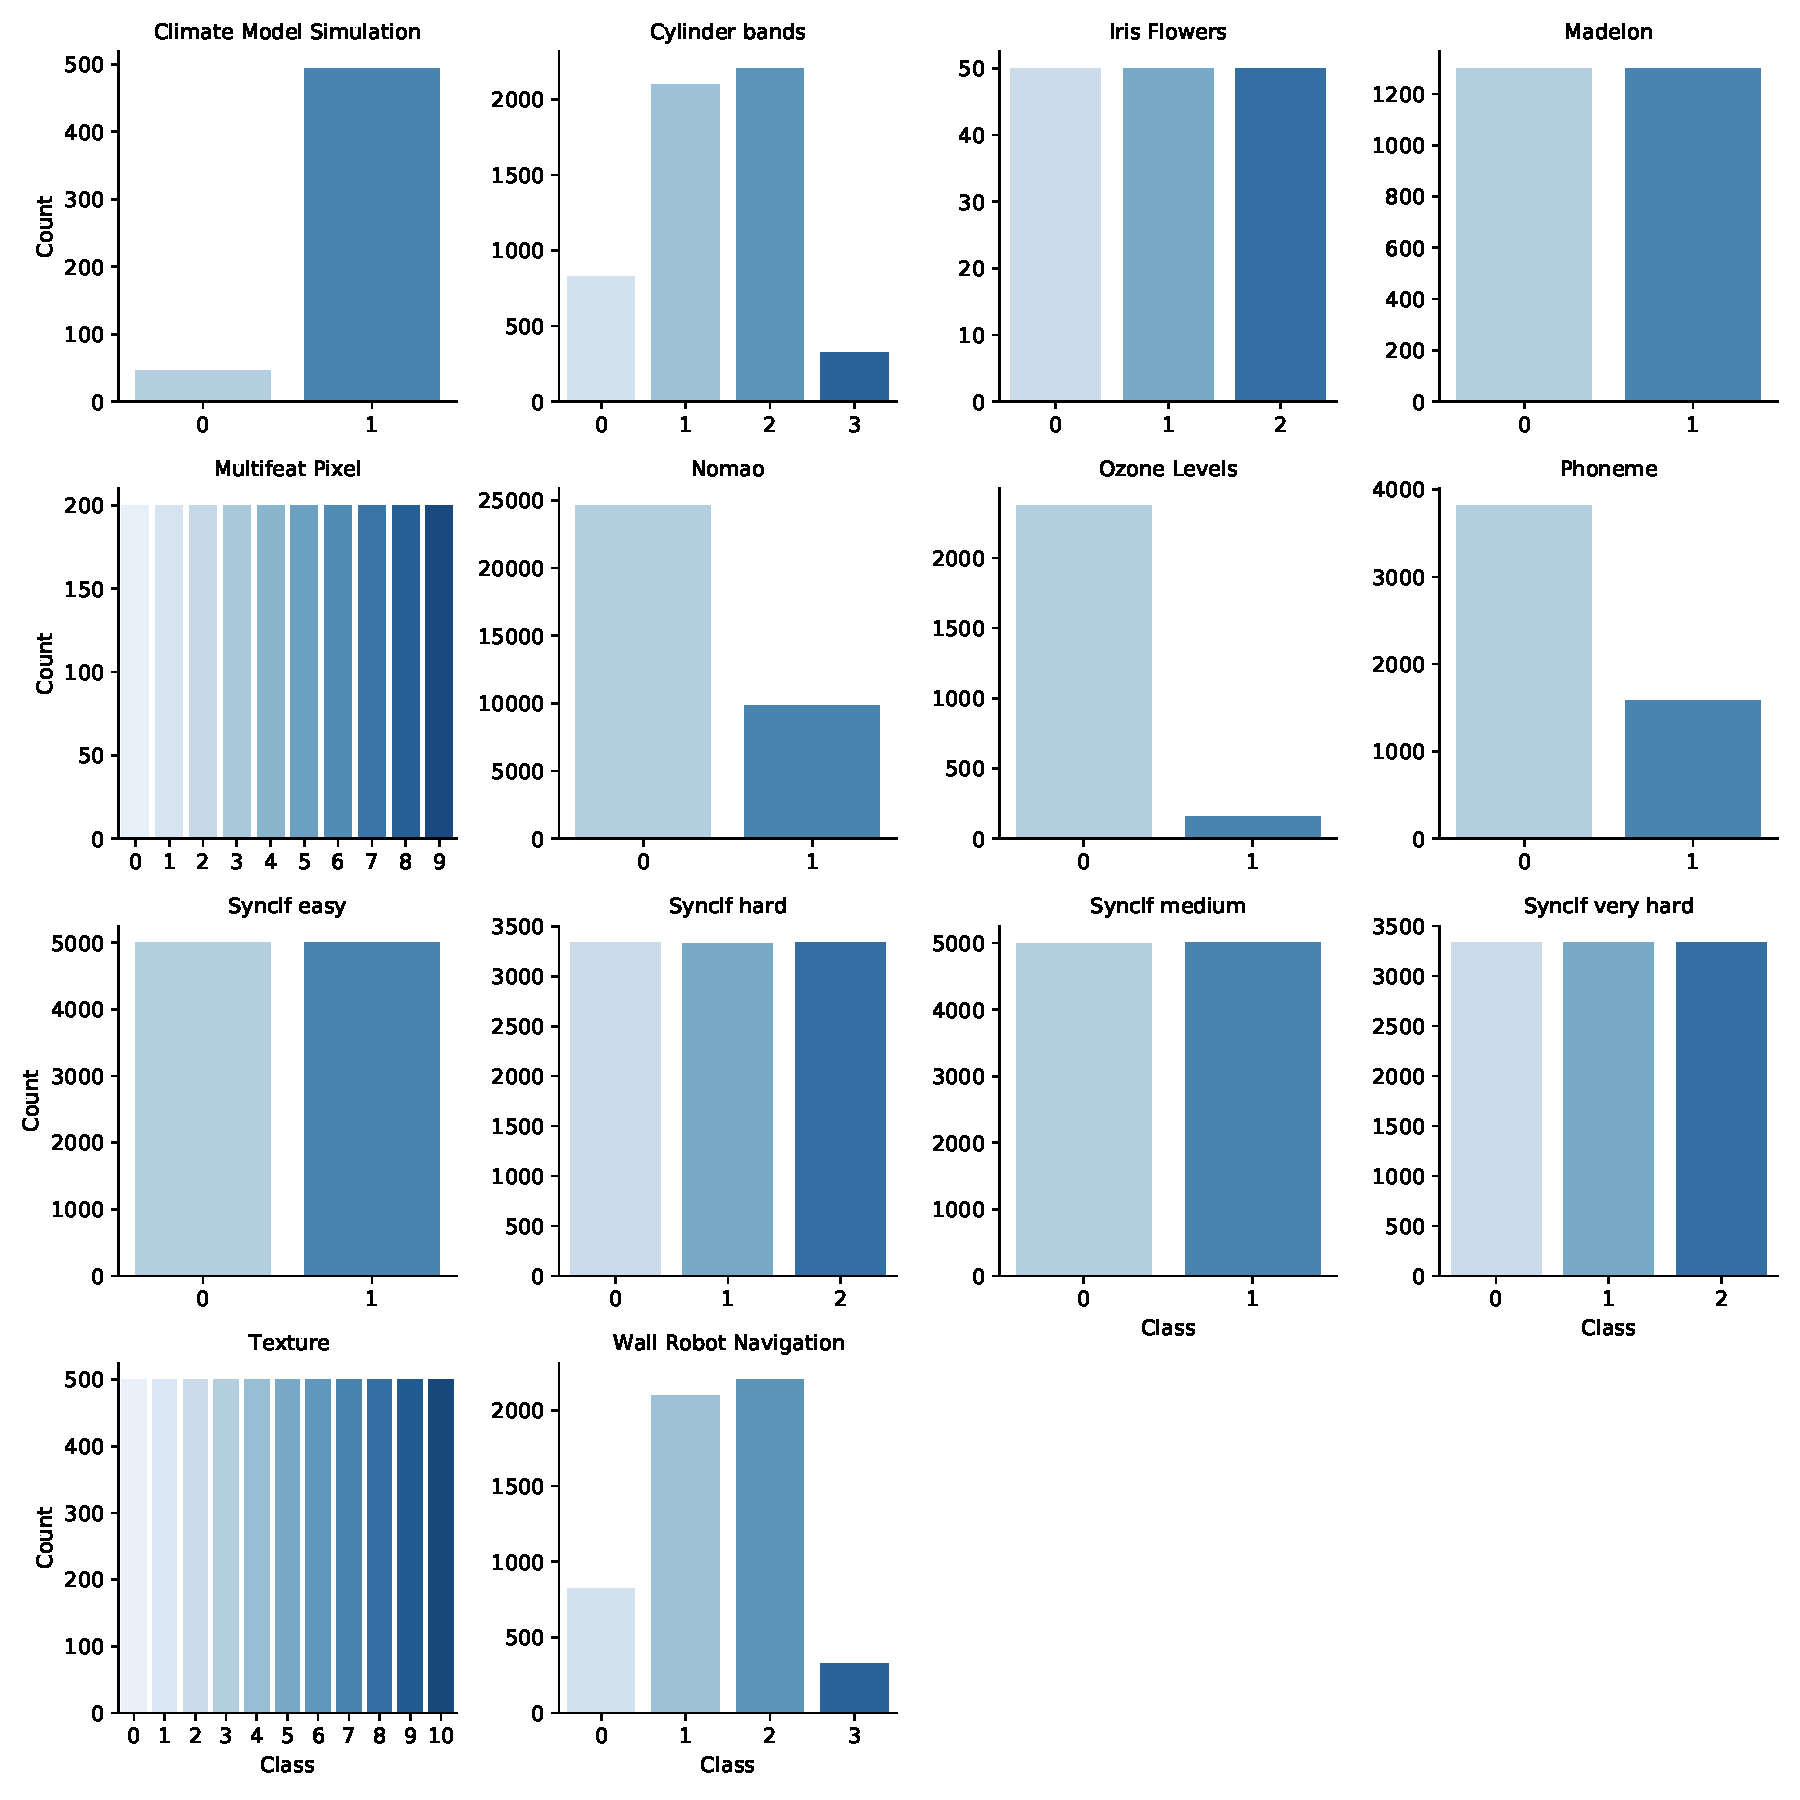
\includegraphics[width=\linewidth]{report/images/experiments_datasets_class_distributions.pdf}
    \caption{Class-distributions of the classification datasets described in Table~\ref{table:experiments-dataset-specification}. The x-axis shows the target classification classes and the y-axis shows the amount of samples with that target class. No binning was applied, the distributions are like shown.}
    \label{fig:experiments-datasets-class-distributions}
\end{figure}



\clearpage
\section{Additional results}\label{section:appendix-additional-results}

\begin{figure}[ht]
    \centering
    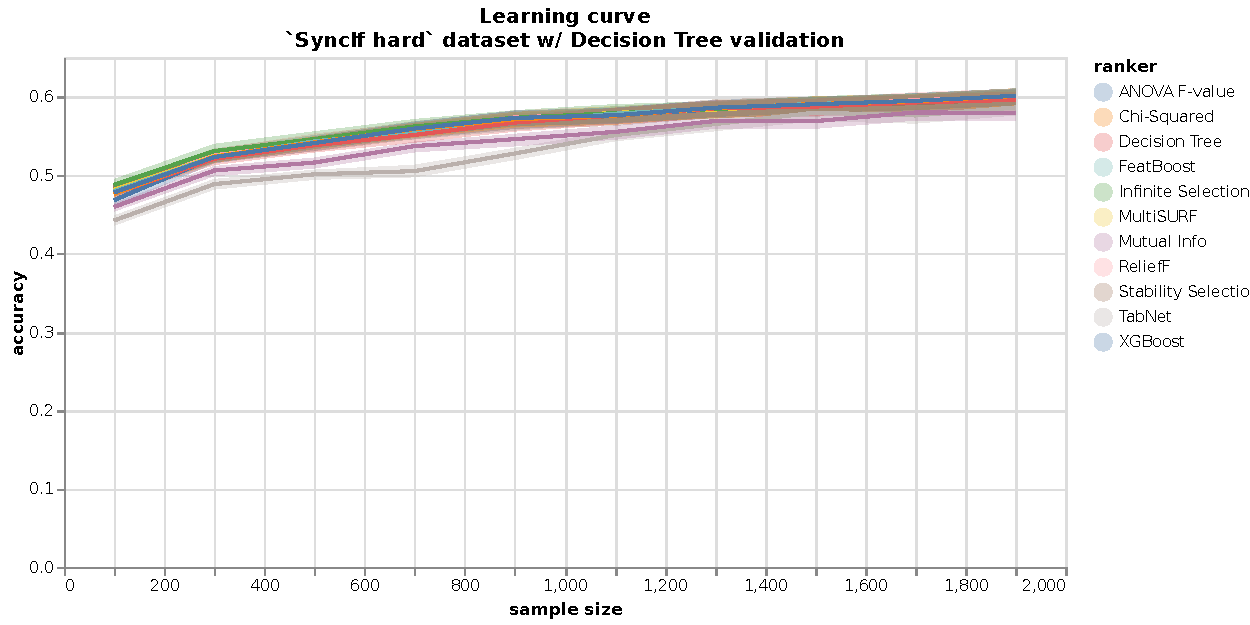
\includegraphics[width=\linewidth]{report/images/results-learning-curve.pdf}
    \caption{Learning curve for `Synclf hard' dataset. Sample sizes from 100 to 2,100 were used, with intervals of 200. The average accuracy over 10 bootstraps is shown.}
    \label{fig:results-learning-curve}
\end{figure}


\begin{figure}[ht]
    \centering
    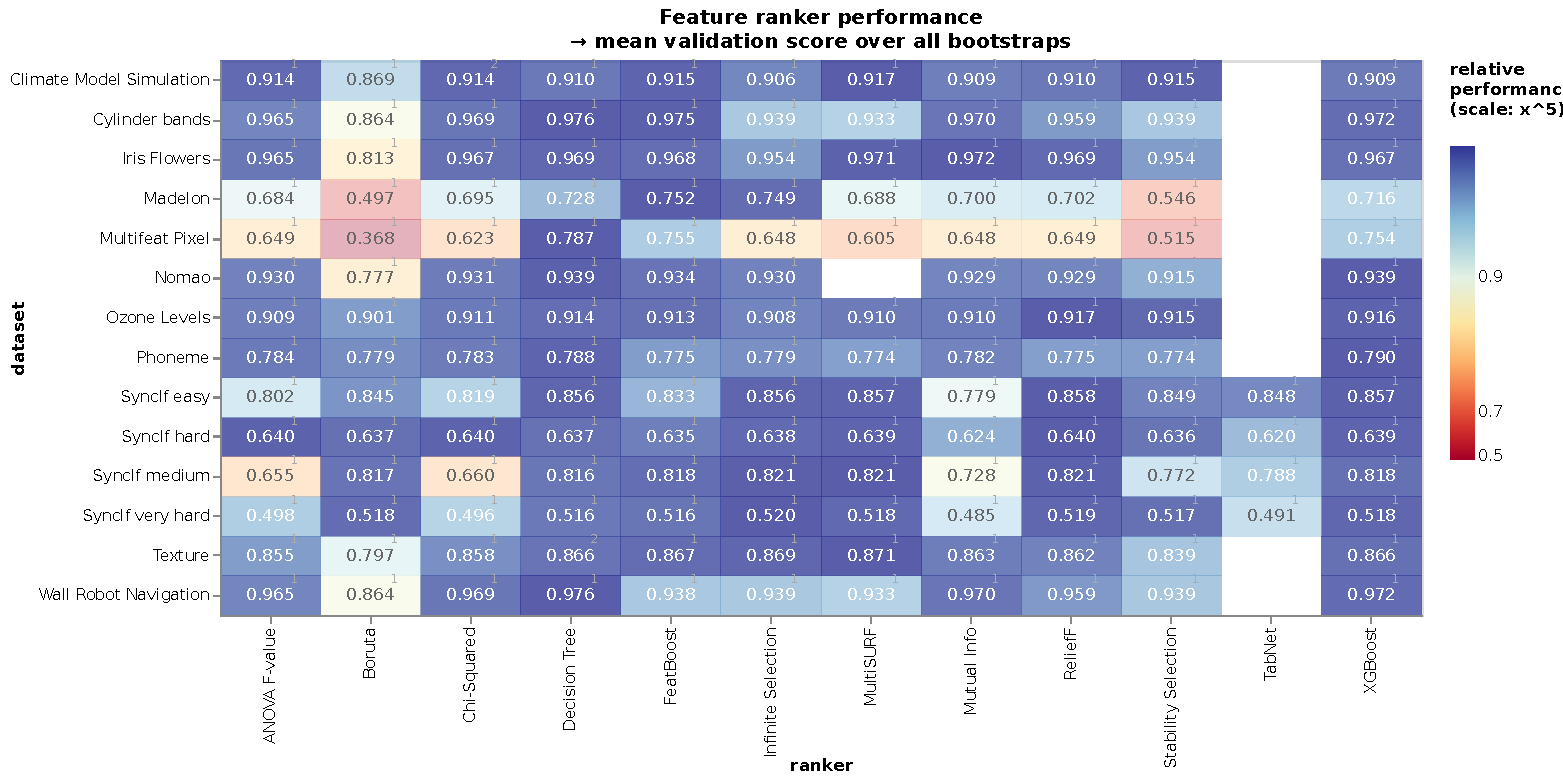
\includegraphics[width=\linewidth]{report/images/results-all-datasets-mean-validation-knn.pdf}
    \caption{\textbf{\gls{knn}} mean validation scores for all datasets. Color scale is configured with \textit{relative performance}, like explained in Section~\ref{section:experiments-example}.}
    \label{fig:results-all-datasets-mean-validation-knn}
\end{figure}


\biblio
\end{document}
